\section{Introduction}
\label{AABB_tree_section_intro}

The AABB tree component offers a static data structure and algorithms to perform efficient intersection and distance queries against sets of finite 3D geometric objects. The set of geometric objects stored in the data structure can be queried for intersection detection, intersection computation and distance. The intersection queries can be of any type, provided that the corresponding intersection predicates and constructors are implemented in the traits class. The distance queries are limited to point queries.\\

Examples of intersection queries include line objects (rays, lines, segments) against sets of triangles, or plane objects (planes, triangles) against sets of segments. An example of a distance query consists of finding the closest point from a point query to a set of triangles.\\

The AABB tree data structure takes as input an iterator range of geometric data, which is then converted into primitives. From these primitives a hierarchy of axis-aligned bounding boxes (AABBs) is constructed and used to speed up intersection and distance queries (see Figure~\ref{fig:AABB-tree-anchor}). 
Each primitive gives access to both one input geometric object (so-called datum) and one reference id to this object. A typical example primitive wraps a 3D triangle as datum and a face handle of a polyhedral surface as id. Each intersection query can return the intersection objects (e.g., 3D points or segments for ray queries) as well the as id (here the face handle) of the intersected primitives. Similarly, each distance query can return the closest point from the point query as well as the id of the closest primitive. 

% AABB tree over anchor triangle surface mesh model.
\begin{center}
    \label{fig:AABB-tree-anchor}
    \begin{ccTexOnly}
      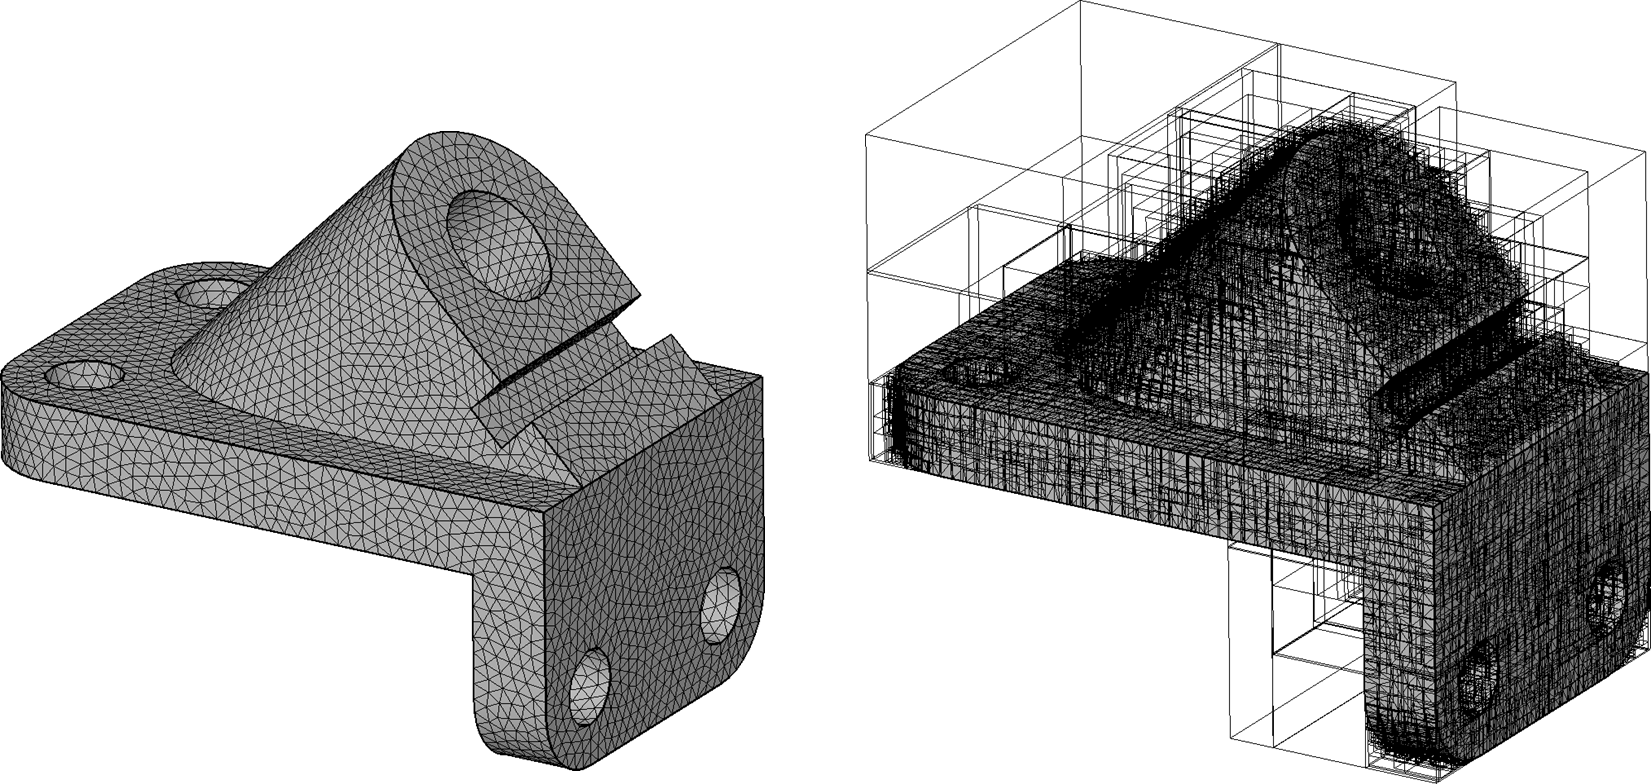
\includegraphics[width=1.0\textwidth]{AABB_tree/figs/anchor}
    \end{ccTexOnly}
    \begin{ccHtmlOnly}
        <img width="99%" border=0 src="./figs/anchor.png"><P>
    \end{ccHtmlOnly}
    \begin{figure}[h]
        \caption{AABB tree.
                 Left: surface triangle mesh of a mechanical part.
                 Right: AABB tree constructed.}
    \end{figure}
\end{center}
